\chapter{Reconstruction}

How do we turn electrical signals into physics.

\section{Tracks}

\section{Primary Vertex}

\section{Particle Flow}

\section{Photons}
\label{sec:photons}

We select high-\ET\ photons from the ECAL Barrel. First, we apply the following cuts to select high-\ET\ photon candidates:
\begin{itemize}
\item Super cluster $\ET > 175\GeV$
\item Super cluster $|\eta| < 1.4442$ .
\end{itemize}
We use the uncorrected \ET\ of the supercluster as photon \ET. 
The use of supercluster raw \ET\ is motivated by an observation that this energy correction causes photon objects with large cluster shower width to exhibit unphysical energies. 
Figure~\ref{fig:corr_vs_sieie} is a profile of the magnitude of the energy correction in bins of \sieie. 
As an illustration, an unphysically large correction is causing the transverse momentum of the photon object in the event shown in Fig.~\ref{fig:badcorr_evtdisp} to be nearly twice as large as the \met, which is supposed to balance the visible, \ie, photon momentum. 
Photon objects with wide showers are used to estimate the hadron-to-photon misidentification background, while the photon energy resolution has an insignificant effect. 
Therefore, unbiased supercluster energy was chosen over the corrected photon energy.

\begin{figure}[htbp]
  \begin{center}
    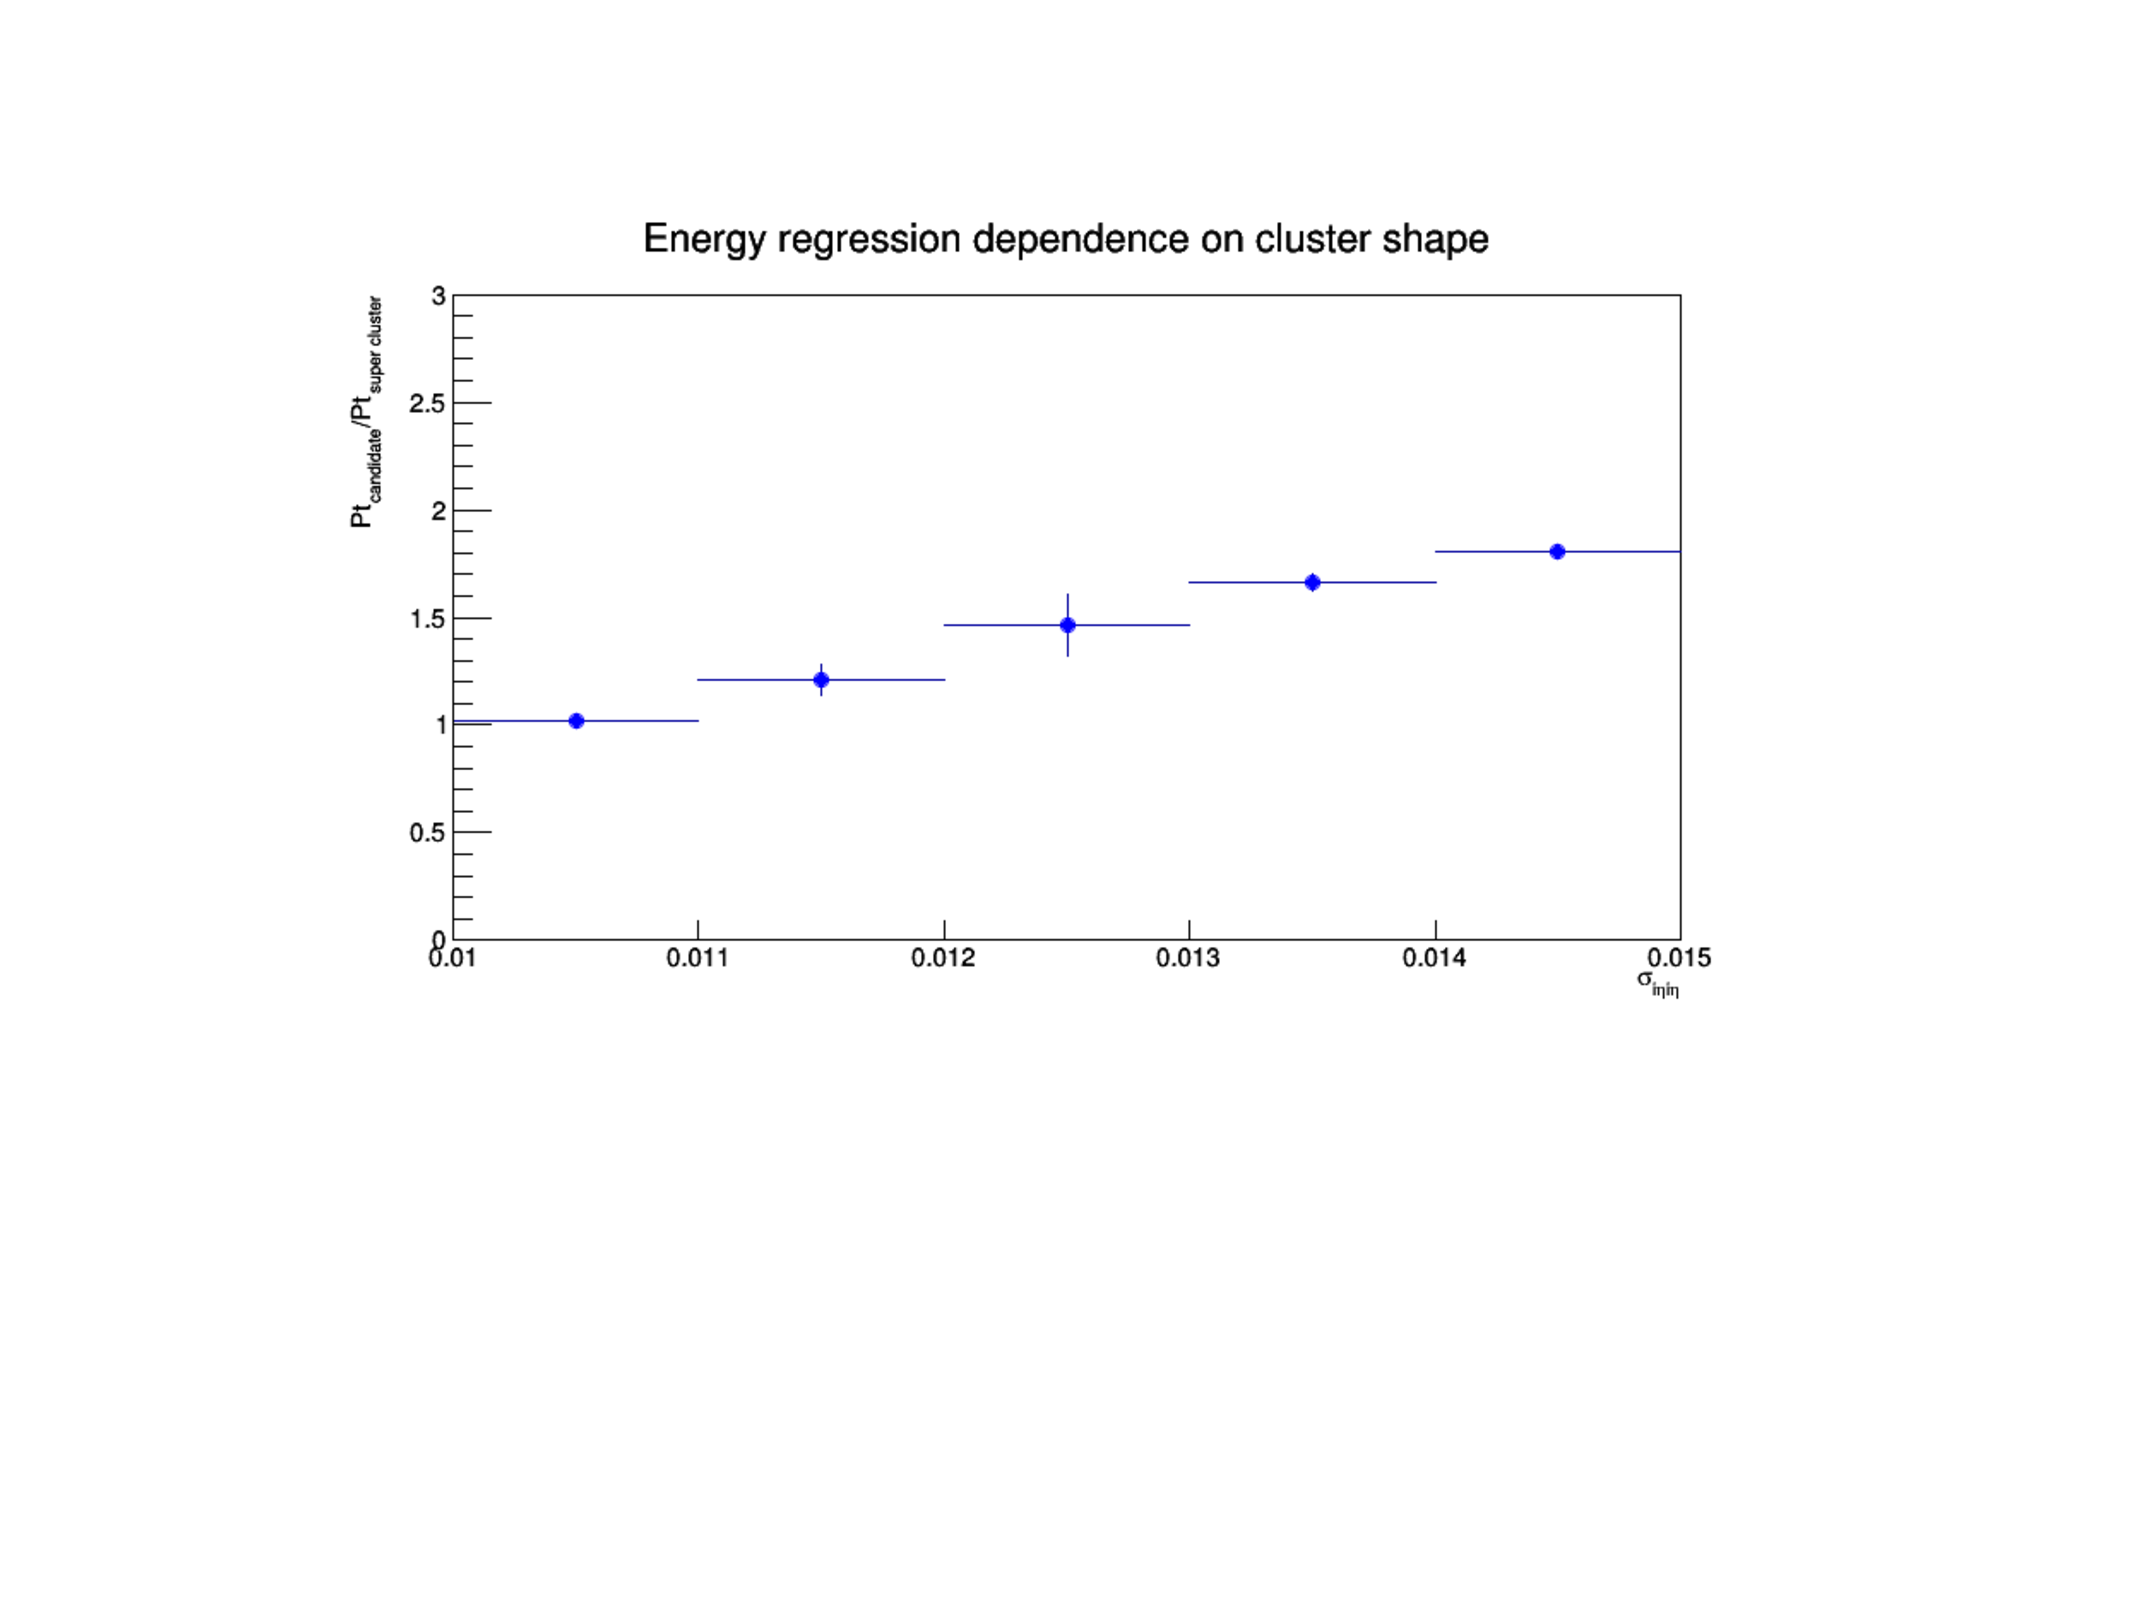
\includegraphics[width=0.6\textwidth]{Reconstruction/Figures/corr_vs_sieie.pdf}
    \caption{
      Magnitude of the energy correction on the photon object in bins of \sieie.
    }
    \label{fig:corr_vs_sieie}
  \end{center}
\end{figure}

\begin{figure}[htbp]
  \begin{center}
    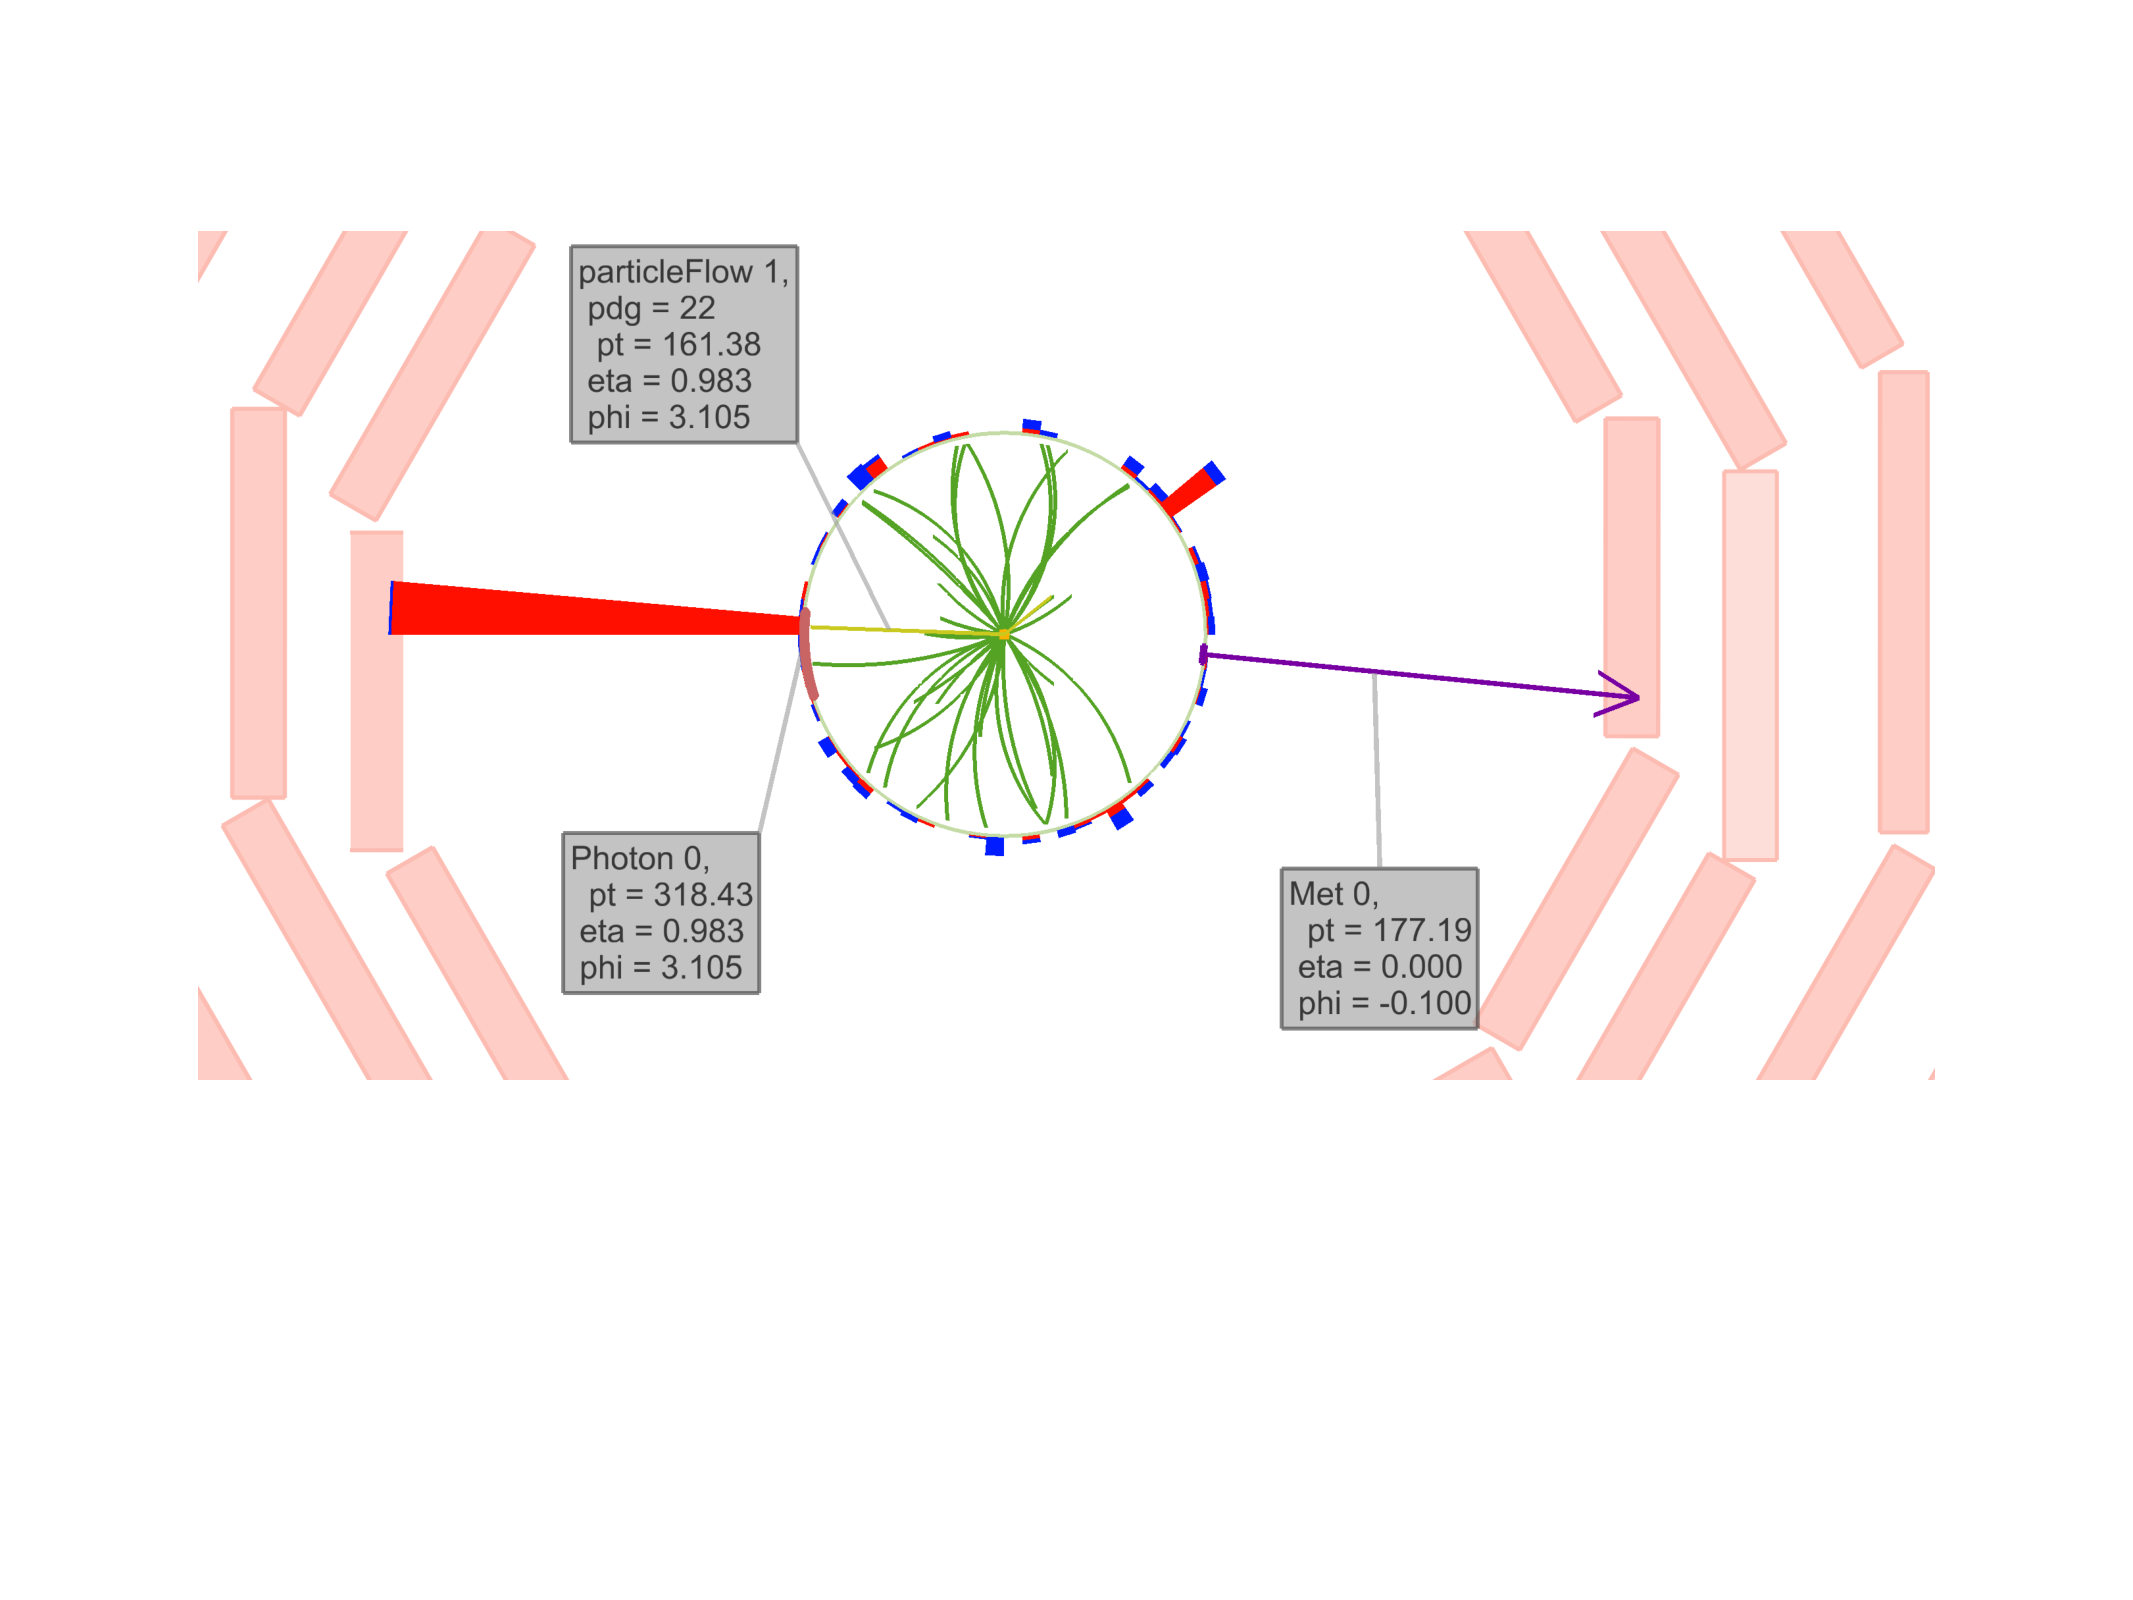
\includegraphics[width=0.6\textwidth]{Reconstruction/Figures/badcorr_evtdisp.pdf}
    \caption{
      An example event where a photon with a wide shower receives a large energy correction.
    }
    \label{fig:badcorr_evtdisp}
  \end{center}
\end{figure}

To reduce hadron-to-photon misidentification rate, we apply the following collection of isolation and shower shape cuts, which will hereby be referred to as the \eg\ ID: 
\begin{itemize}
  \item $H/E < 0.0260$
  \item $\sieie < 0.01040$
  \item $\rho$-corrected maximum PF charged hadron isolation $\ICHmax < 1.146\GeV$
  \item $\rho$-corrected PF neutral hadron isolation $\INH < 2.792\GeV + 0.0112 \times \ETg + 0.000028 \times \left(\ETg \right)^2/\GeV$
  \item $\rho$-corrected PF photon isolation $\Ig < 2.176\GeV + 0.0043 \times \ETg$
\end{itemize}

In the identification criteria, the maximum PF charged hadron isolation \ICHmax\ is the maximum of the standard PF charged hadron isolation computed for all reconstructed vertices. 
Standard PF charged hadron isolation is computed with respect to the primary vertex. 
Since the object with the highest \pt\ in the selected events is typically a photon, which has no intrinsic association to a vertex, it is possible that the identified primary vertex does not correspond to the \Pp\Pp\ interaction from which the photon object originate. 
In such cases, the photon object can be surrounded by charged hadrons, \ie, a part of a jet, and still appear isolated under the standard charged hadron isolation. 
The use of maximum isolation is a conservative measure to address such misidentification.

Effective areas for isolations are also recomputed to maintain flat pileup dependence as given in Table~\ref{tab:ea}
%
\begin{table}[htbp]
  \begin{center}
    \caption{Effective areas for isolations.} 
    \label{tab:ea}
    \begin{tabular}{|c|c|c|}
      \hline
      Isolation & $|\eta|<1.0$ & 1.0$<|\eta|<1.479$  \\
      \hline
      maximum PF charged hadron isolation & 0.01064& 0.1026 \\
      PF neutral hadron isolation & 0.0597 & 0.0807 \\
      PF photon isolation & 0.1210 & 0.1107 \\
      \hline
    \end{tabular}
  \end{center}
\end{table}

To reject electrons from the candidate sample, we require that no electron track seeds can be associated to the super cluster. This is known as the pixel seed veto.

To clean the candidate sample from photon objects originating from non-collision sources. we apply the following collection of cuts, which combined with the pixel seed veto constitutes the \Pgg\-specific ID:
\begin{itemize} 
  \item Beam halo tagger $\emip < 4.9\GeV$
  \item $\sieie > 0.001$
  \item $\sipip > 0.001$
  \item Cluster seed time $|\tseed| < 3\ns$ .
\end{itemize}
Beam halo tagger is the total energy deposited in ECAL by a hypothetical beam halo muon that passes through the photon cluster. 
Lower bounds for \sieie\ and \sipip\ as well as the requirement on the cluster seed time are employed to reject spurious photon objects arising from ``ECAL spikes'', or anomalous electronic signal induced at the ECAL Barrel photodetectors by nuclear or ionizing interactions in the photocathode.

\section{Electrons}

\section{Muons}

\section{Hadrons and jets}

\subsection{Hadronic taus}

\section{Missing Transverse Energy}

\iffalse
\section{Non-collision signatures}

Things that don't come from protons.

\subsection{Beam halo}

\subsection{ECAL Spikes}

\subsection{Fake MET}
\fi
